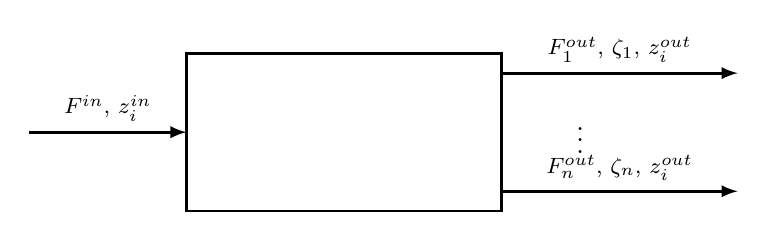
\begin{tikzpicture}[arrow/.style={line width=1pt,->,>=latex}]
	\draw [line width=1pt] (-2,2) rectangle (2,0);
	\draw [arrow] (-4,1) -- (-2,1) node [pos=0.5, above] {\footnotesize $F^{in}$, $z_i^{in}$};
	\draw [arrow] (2,1.75) -- (5,1.75) node [pos=0.5, above] {\footnotesize $F_1^{out}$, $\zeta_1$, $z_i^{out}$};
	\node at (3,1) {\vdots};
	\draw [arrow] (2,0.25) -- (5,0.25) node [pos=0.5, above] {\footnotesize $F_n^{out}$, $\zeta_n$, $z_i^{out}$};
\end{tikzpicture}